\documentclass[a4paper, 12pt]{article}
\usepackage{graphicx}

\renewcommand{\thesubsection}{\thesection.\alph{subsection}}


\usepackage{xparse}
\ExplSyntaxOn
\NewDocumentCommand{\Rowvec}{ O{,} m }
{
	\vector_main:nnnn { p } { & } { #1 } { #2 }
}
\NewDocumentCommand{\Colvec}{ O{,} m }
{
	\vector_main:nnnn { p } { \\ } { #1 } { #2 }
}

\seq_new:N \l__vector_arg_seq
\cs_new_protected:Npn \vector_main:nnnn #1 #2 #3 #4
{
	\seq_set_split:Nnn \l__vector_arg_seq { #3 } { #4 }
	\begin{#1matrix}
		\seq_use:Nnnn \l__vector_arg_seq { #2 } { #2 } { #2 }
	\end{#1matrix}
}
\ExplSyntaxOff

\usepackage{enumitem}
\usepackage{t1enc}
\usepackage[utf8]{inputenc}
\usepackage[magyar]{babel}

% a szép matematikai szimbólumokért
\usepackage{amssymb}
\usepackage{amsmath}
\usepackage{nccmath}
\usepackage{siunitx}

\usepackage{listings}
\lstset{language=Python}

\usepackage{subcaption}
\usepackage[justification=centering]{caption}

% ha táblázatban szeretnénk egyesített sorokat is
\usepackage{multirow}

% horizontal line
\usepackage{hhline}

% eps formátumú ábrák --> pdflatex fordításhoz!!
\usepackage{epsfig}

% egyenletekhez, pl mátrixok írására
\usepackage{array}

% ha betűszíneket is szeretnénk használni
\usepackage{color}

% Margók egyéni beállításai
\usepackage{anysize}
\marginsize{1.64cm}{1.64cm}{1.2cm}{2.4cm} %\left right top bottom

% vakszöveg
\usepackage{lipsum}
\usepackage{blindtext}

% A HIVATKOZÁSOKHOZ HASZNÁLT CSOMAGOK. RÉSZLETESEBBEN LD: google -> latex bibtex
\usepackage[numbers, square, comma, sort&compress]{natbib}
%\usepackage[format=hang,labelsep=period]{caption}

\usepackage[unicode]{hyperref}   % ezzel a hivatkozások linkké válnak
\usepackage{bookmark}
\hypersetup{bookmarksopen={true}}
\hypersetup{bookmarksopenlevel={2}}
\hypersetup{bookmarksnumbered={true}}
\hypersetup{
	colorlinks,%
	citecolor=red,%
	filecolor=black,%                                                                                                                                               
	linkcolor=blue,%
	urlcolor=green
}
\numberwithin{equation}{section}          % ezekkel tudod beállítani, hogy milyen felbontásig menjen a hivatkozás
\numberwithin{figure}{subsection}
%\numberwithin{table}{section}          % ha kikommenteled, akkor csak simán számozva lesz.

%%%%%%%%%%%%%%%% Néhány dolog a fancy kinézethez

\frenchspacing
\setlength{\parskip}{2ex}
\setlength{\headsep}{0,4cm}
\setlength{\headheight}{4pt}

% fej- es lábléc
\usepackage{fancyhdr}
\usepackage{fancyref}
\usepackage{fancyvrb}
\pagestyle{fancy}

\renewcommand{\headrulewidth}{0,05pt}
\renewcommand{\footrulewidth}{0pt}


\fancyhf{}
\fancyhead[LO]{{ \nouppercase{\rightmark}} }

\cfoot{--~\thepage~--}

%%%%%%%%%%%%%%%%%%%%%%%%%%%


%%%%%%%%%%%%%%%%%%%%%%%%%%%%%%%%%%%%%%%%%%%%%%%%%%%%%%%%%%%%%%%%%%%%%%%%%%%%

\begin{document}

% Címoldalt lehet egyszerűen a \maketitle paranccsal is. Ha kissé részletesebb
% címre van szükség, azt lehet így is, kézzel megadva mindent.
\begin{titlepage}   
\begin{center}
\thispagestyle{empty}  

\vspace*{0.7cm}
\rule{\linewidth}{0.5mm} \\[3mm]
\vspace*{0.7cm}

{\LARGE Véletlen fizikai folyamatok}

\vspace*{0.7cm}
\rule{\linewidth}{0.5mm} \\[3mm]
\rule{\linewidth}{0.5mm} \\[3mm]



{\Large 6. beadandó\\}

\vspace*{0.7cm}
\rule{\linewidth}{0.5mm} \\[3mm]
  {\small Márton Tamás} \\[3mm]
{\footnotesize PJF19C} \\
{\footnotesize martontamas@caesar.elte.hu}

  \vspace*{2cm}

\begin{figure}[h!]
\begin{center}

\includegraphics[width=0.5\textwidth]{./elte.png}
\end{center}
\end{figure}

\end{center}
\end{titlepage}

\newpage

%%%%%%%%%%%%%%%%%%%%%%%%%%%%%%%%%%%%%%%%%%%%%%%%%%%%%%%%%%%%%%%%%%%%%%%%

\thispagestyle{empty}  

%1
\section{feladat}

\begin{center}
\underline{Feladat leírás.}
\end{center}

Csön-csön gyűrűt játszanak hárman. A gyűrűt a körben álló játékosok az óramutató járásával egy irányban adják tovább. Az 1-es gyereknél indul a gyűrű, s a továbbadási ráta w. \ newline

\begin{enumerate}
	\item Írjuk fel az egyenletet annak a valószínűségére, hogy a gyűrű az $i$-edik gyereknél van!
	\item Határozzuk meg a stacionáris megoldást!
	\item Határozzuk meg a rendszer relaxációs idejét (először próbáljuk megbecsülni az értékét)!
\end{enumerate}


\begin{center}
\underline{Feladat megoldása.}
\end{center}
\hspace{5cm}


\textbf{\textbf{1.}} \newline

Körben ülnek a gyerekek, tehát az 1. gyermek a 3. gyermektől megkaphatja a gyűrűt. Mivel csak az
óramutató járásával egy irányban adják tovább, ezért egy adott állapotból a rendszer csak 1 irányba tud
elmozdulni. Így a Master-egyenlet, ami leírja annak a valószínűségét, hogy az $i.$ gyermeknél van a gyűrű $t$ időpontban:

\begin{center}
	\begin{gather}
	\frac{\partial}{\partial t}P_i(t) = -wP_{i}(t)+wP_{i-1}(t),\   \  i = 1,2,3.
	\end{gather}
\end{center}

Amely a három gyermekre kiírva:

\begin{center}
	\begin{gather*}
	\frac{\partial}{\partial t}P_1(t) = -wP_1(t)+wP_3(t)
	\frac{\partial}{\partial t}P_2(t) = -wP_2(t)+wP_1(t)
	\frac{\partial}{\partial t}P_3(t) = -wP_3(t)+wP_2(t)
	\end{gather*}
\end{center}

Vezessük be a rendszerünket leíró valószínűségi vektort:

\begin{center}
	\begin{gather}
		\vec{P}(t) = \begin{pmatrix}P_1(t)\\P_2(t)\\P_3(t)\end{pmatrix}
	\end{gather}
\end{center}

\newpage
A rendszerünk dinamikai mátrixa pedig a következő:

\begin{center}
	\begin{gather}
	\textbf{A} = \begin{bmatrix}
	-w & 0 & w\\
	w & -w & 0 \\
	0 & w & -w
	\end{bmatrix}
	\end{gather}
\end{center}

ami sztochasztikus, hiszen minden oszlopban a tagok összege zérus. Mivel e mellé még az állapottér irreducibilis is, a Perron–Frobenius-tétel kimondja, hogy az A dinamikai mátrixunk legkisebb és legnagyobb
sajátértéke nem degenerált. Biztos, hogy van egy $\lambda_1$ sajátértéke a mátrixnak ami nulla, a többinek a valós része viszont mind negatív, hiszen a rendszer különben elszállna. A stacionárius megoldáshoz a
$\lambda_1 = 0$ sajátértékhez tartozó sajátvektorra van szükségünk, amit egy sajátérték számolásra alkalmas \href{http://matrixcalc.org/en/}{weboldal} segítségével
számoltam ki:

\begin{center}
	\begin{gather}
	\left( \textbf{A} -\lambda_1 \right)\vec{P}^{(e)} = 0 \rightarrowtail  \vec{P}^{(e)} = \frac{1}{3}\begin{pmatrix}1\\1\\1\end{pmatrix}
	\end{gather}
\end{center}


Az $\frac{1}{3}$ szorzó a normálást mutatja. Azt kaptuk amit vártunk, hiszen egy szimmetrikus problémáról
van szó, egyensúlyban mindegyik állapot ugyanakkora valószínűséggel fordulhat elő. A rendszer relaxációs
idejére  $t = \infty $ és értéket becsülök, hiszen az egyensúlyi állapot számomra egy olyan állapotot jelent, amiből
a rendszer nem akar kimozdulni. És ennél a játéknál ha csak adogatják körbe a gyűrűt, nincs egy külső
kényszer ami a körbeadogatást korlátozná, vagyis mindig mozgásban kell lenni a gyűrűnek. Emellett a
relaxációs időt akár $t = 0$-nak is becsülhetjük, mert igazából abból az állapotból nem fog kimozdulni
a rendszer, hogy folyamatosan adogatják körbe a gyűrűt. Eszerint értelmezés szerint az általam becsült
relaxációs idő vagy $t = \infty $ vagy $t = 0$.

\newpage
%2
\section{feladat}

\begin{center}
\underline{Feladat leírás.}
\end{center}
Végezzünk szimulációkat az egy-dimenziós Ising modell egyensúlyi tulajdonságainak meg-
határozására. A rendszer állapotát egydimenziós rács pontjaiban $(i = 1, 2, ..., N )$ ülő $s_i = \pm 1$
spinek határozzák meg. A spinek szomszédjaikkal ferromágnesesen hatnak kölcsön, azaz egy
állapot energiája a következő:

\begin{center}
	\begin{gather}
		E(s_1,s_2....,s_N) = J \sum_{1}^{N-1}s_is_{i+1}, \  \ J>0.
	\end{gather}
\end{center}

A spinek $T$ hőmérsékletű környezettel vannak kölcsönhatásban, s ennek eredményeképpen
átbillenhetnek egyik állapotukból a másikba $(s_i \Leftrightarrow -s_i )$.
Válasszunk spin-flip rátának olyan alakot, ami kielégíti a részletes egyensúly elvét. Ilyen
lesz például, ha az $i$-edik spin forgatásának ($s_i \rightarrow -s_i $) rátája a következő ($1/s$ egységben):

\begin{center}
	\begin{gather}
	w(s_1,...,s_{i-1},s_i,s_{i+1,...s_N}) =
	\begin{cases}
	1       & \quad ha\ \ \Delta E < 0\\
	1/2     & \quad ha\ \ \Delta E = 0 \\
	e^{(-\beta \Delta E)}  & \quad ha\ \ \Delta E > 0 \\
	\end{cases}        
	\end{gather}
\end{center}
ahol, mint könnyen belátható
\begin{center}
	\begin{equation}
\Delta E = 2Js_i(s_{i-1} + s_{i+1}).
	\end{equation}
\end{center}

Legyen $N = 50$, s kezdjük a rendszer szimulálását teljesen véletlenszerű állapotból, ahol
$1/2$ valószínűséggel $s_i = \pm 1$ (az egyensúlyi átlagok nem függhetnek a kezdeti feltételtől, tehát
eredményeink helyességét ellenőrizhetjük azzal, hogy teljesen rendezett állapotból indítjuk a
rendszert, s megnézzük ugyanazt kapjuk-e).

\newpage
A szimuláció lépései:

\begin{enumerate}
	\item Véletlenszerűen kiválasztunk egy spint.
	\item Megnézzük, hogy ha megforgatjuk, akkor mennyit változik a rendszer energiája, azaz kiszámítjuk $\Delta E$-t.
	\item Ha $\Delta E < 0$, akkor megforgatjuk a spint, és megyünk az $(1)$-es ponthoz
	\item Ha $\Delta E = 0$, akkor húzunk egy véletlen számot $P$-t a $[0, 1]$ intervallumból, és ha $P < 1/2$, akkor megforgatjuk a spint, s megyünk az $(1)$-es ponthoz. Ha $P > 1/2$, akkor forgatás
	nélkül megyünk az $(1)$-es ponthoz
	\item Ha $\Delta E > 0$, akkor húzunk egy véletlen számot $P$-t a $[0, 1]$ intervallumból, és ha $P <
	e^(-\beta \Delta E)$, akkor megforgatjuk a spint, egyébként megyünk az $(1)$-es ponthoz.
\end{enumerate}

Az $(1)-(5)$ pontokat sokszor, $N \cdot t$-szer elvégezve azt mondjuk, hogy $t$ idő telt el. Minden
rendszernek van általában egy relaxációs ideje, $\tau$ , és ha $t > \tau $ , akkor a rendszer elérkezik az
egyensúlyba, és attól kezdve a különböző mennyiségek, mint például a mágnesezettség

\begin{center}
	\begin{gather}
		m = \frac{1}{N} \sum_{i = 1}^{N}s_i,
	\end{gather}
\end{center}

vagy a mágnesezettség fluktuációja $m_2$ , az egyensúlyi értéke körül fluktuál. Az egyensúlyi
átlagokat $(\langle m \rangle, \rangle m^2 \rangle)$ tehát megbecsülhetjük mint időátlagokat. Ez azt jelenti, hogy $t_1$
időnként kiszámítjuk (megmérjük) az $m$ és az $m_2$ értékét, majd elég sok ilyen mérésből
átlagokat számolunk, s ezek megadják a $T$ hőmérsékleti termodinamikai átlagokat, $\langle m \rangle$-t és
$\langle m^2 \rangle$-t.
\newline

Határozzuk meg az $\langle m \rangle$ és az $\langle m^2 \rangle$ átlagokat az alábbiakban megadott egyéni $\beta J$ értékeknek megfelelő hőmérsékleteken. Próbáljuk megmagyarázni az eredményt! Mentsünk el egy-
egy egyensúlyi spinkonfigurációt $\{s_1 , ..., s _{i-1} , s_i , s_{i+1} , ..., s 50 \}$ mind a négy $\beta J$ értéknél, egy
későbbi feladatban esetleg szükség lesz rájuk.

\newpage
\begin{center}
	\underline{Feladat megoldása.}
\end{center}


A szimulációs problémát Python nyelven oldottam meg, jupyter-notebookban. Legelőször importáltam a szükséges csomagot a matematikai műveletekhez és az ábrázoláshoz, majd egy tömbben eltároltam a személyre
szabott paramétereim, illetve deklaráltam, hogy $N = 150$ darab spint fogok szimulálni:
\newline
\rule{\textwidth}{0.1pt}
\begin{lstlisting}
%pylab inline

BetaJ = [0.12, 0.24, 0.75, 1.60]
N = 150 
\end{lstlisting}
\rule{\textwidth}{0.1pt}

A szimuláció során a $J$ paraméter értékét végig 1-nek vettem. Ezek után írtam egy függvényt az adott
spinkonfiguráció energiájának kiszámítására:
\newline
\rule{\textwidth}{0.1pt}
\begin{lstlisting}
def E(spinek):
	s = 0
	for i in range(1, len(spinek)):
		s = s + spinek[i-1] * spinek[i]
	E = -s
	return E
\end{lstlisting}
\rule{\textwidth}{0.1pt}

Majd megírtam az energiakülönbség kiszámítására is a kellő függvényt:
\newline
\rule{\textwidth}{0.1pt}
\begin{lstlisting}
def dE(s0 ,s1, s2):
	return 2 * s1* (s0 + s2)
\end{lstlisting}
\rule{\textwidth}{0.1pt}

\newpage
Mindezek után implementáltam a szimuláció léptető függvényét. Ezen felül látható a kódból, hogy alkalmaztam egy periodikus határfeltételt annak
érdekében, hogy tudjuk kezelni azokat az eseteket, ha az első, vagy esetleg az utolsó spint választanánk:
\newline
\rule{\textwidth}{0.1pt}
\begin{lstlisting}

def Leptetes(s, N, BetaJ):
	rand = random.randint(0, N) 


	if rand == 0:
		s1 = s[rand]
		s0 = s[N-1]
		s2 = s[rand+1]


	if rand == N-1:
		s1 = s[rand]
		s0 = s[rand-1]
		s2 = s[0]
	else:
		s0 = s[rand-1]
		s1 = s[rand]
		s2 = s[rand+1]


	if dE(s0, s1, s2) < 0:
		s[rand]= -s[rand]
		return s


	elif dE(s0, s1, s2) == 0:
		P = random.random()
		if P < 0.5:
			s[rand]= -s[rand]
			return s
		else:
			return s


	else: 
		P = random.random()
		if P < exp(-BetaJ * dE(s0, s1, s2)):
			s[rand] = -s[rand]
			return s
		else:
			return s

\end{lstlisting}


Ezek segítségével elvégeztem a szimulációt:
\newline
\rule{\textwidth}{0.1pt}
\begin{lstlisting}
s = (random.randint(0, 2, (N,)) -1/2) * 2   
b = 0                             
t = 1000                                    
m = []                                      


sFrissitett = s
for i in range(N*t):
	s = sFrissitett
	m.append(sum(s) / N)    
	sFrissitett = Leptetes(s, N, BetaJ[b])
\end{lstlisting}
\rule{\textwidth}{0.1pt}

Ezek után minden $\beta J$ értékre $5$-ször lefuttattam a szimulációt, és táblázatba írtam  az aktuális $m$ mágnesezettséget a szimuláció legvégén, az átlagos $\langle m \rangle$ mágnesezettséget, illetve az
átlagos mágnesezettség szórásnégyzetét, úgy mint $\langle m^2 \rangle - \langle m \rangle^2$ . A négy futtatás eredményeit kiátlagoltam,
és az átlag hibáját úgy adtam meg, hogy:

\begin{center}
	\begin{equation}
		\sigma^2= \frac{1}{n}\sum_{i=1}^{n}\left( x_i - \langle x \rangle \right)^2 \rightarrowtail \sigma = \sqrt{\sigma^2} 
	\end{equation}
\end{center}

\begin{center}
	\begin{tabular}{ ||c|c|c|c|| } 
		\hline
		Szimuláció &  m & $\langle m \rangle$ & $\langle m^2 \rangle$- $\langle m \rangle^2$\\ 
		\hline
		1 & -0.026667  & -0.002580 & 0.009245\\
		2 &  0.013333 & -0.001022 & 0.008111\\
		3 &  -0.053333 & -0.006363 & 0.008668\\
		4 &  0.106667 & 0.002168 & 0.008631\\
		5 &  0.013333 & -0.001479 & 0.007973\\
		\hline
		Átlagok & 0.01066659$\pm$ 0.0960004 & 0.0018552 $\pm$0.0045078 & 0.008637$\pm$0.0006079 \\
		\hline
	\end{tabular}\par
\bigskip
$\beta J = 0.12, szimuláció eredményei.$
\end{center}


\begin{center}
	\begin{tabular}{ ||c|c|c|c|| } 
		\hline
		Szimuláció &  m & $\langle m \rangle$ & $\langle m^2 \rangle$- $\langle m \rangle^2$\\ 
		\hline
		1 & 0.106667  & 0.003185 & 0.011440\\
		2 &  -0.146667 & 0.006580 & 0.010222\\
		3 &  0.173333 & -0.002153 & 0.010128\\
		4 &  0.093333 & 0.005341 & 0.010224\\
		5 &  0.120000 & 0.001454 & 0.010791\\
		\hline
		Átlagok & 0.346666$\pm$ 0.493333 & 0.014407$\pm$0.006580 & 0.041365$\pm$0.052156 \\
		\hline
	\end{tabular}\par
	\bigskip
	$\beta J = 0.24, szimuláció eredményei.$
\end{center}


\begin{center}
	\begin{tabular}{ ||c|c|c|c|| } 
		\hline
		Szimuláció &  m & $\langle m \rangle$ & $\langle m^2 \rangle$- $\langle m \rangle^2$\\ 
		\hline
		1 & -0.173333  & -0.032539 & 0.034690\\
		2 &  0.040000 & 0.007498 & 0.033385\\
		3 &  -0.200000 & -0.015977 & 0.032477\\
		4 &  -0.306667 & -0.052809 & 0.023548\\
		5 &   0.226667 & 0.000260 & 0.024044\\
		\hline
		Átlagok & -0.082666$\pm$ 0.309333 & -0.0187134$\pm$0.0340956 & 0.0296288$\pm$0.0037562\\
		\hline
	\end{tabular}\par
	\bigskip
	$\beta J = 0.75, szimuláció eredményei.$
\end{center}


\begin{center}
	\begin{tabular}{ ||c|c|c|c|| } 
		\hline
		Szimuláció &  m & $\langle m \rangle$ & $\langle m^2 \rangle$- $\langle m \rangle^2$\\ 
		\hline
		1 & -0.346667  & 0.453322 & 0.060846\\
		2 &  0.146667 & 0.453322 & 0.043041\\
		3 &  0.106667 & 0.419848 & 0.028452\\
		4 &  0.453333 & 0.138696 & 0.130770\\
		5 &   0.240000 & 0.115783 & 0.141747\\
		\hline
		Átlagok & 0.12$\pm$ 0.226667 & 0.2428866$\pm$0.086784 & 0.068802$\pm$0.072945\\
		\hline
	\end{tabular}\par
	\bigskip
	$\beta J = 1.6, szimuláció eredményei.$
\end{center}


Példaként kiábrázoltam az $m$ mágnesezettség időfüggését a különböző $\beta J$ értékek mellett, ez látható
a $\ref{m}$ ábrán, amiről leolvashatjuk, hogy az m mágnesezettség az $m = 0$ érték körül fluktuál, s nagyobb
kiugrások a legnagyobb $\beta J$ érték esetén tapasztalhatók. Azért nem látunk az ábrán egy jellegzetes "relaxáló" lecsengést, mert a szimulációt random (-1 vagy +1 egyenlő valószínűséggel) spinekkel indítottam,
így már kezdetben is a rendszer $m$ mágnesezettsége $0$ körüli értéket vesz fel. A táblázatokból jól látszik
továbbá, hogy ahogy $\beta J$ értéke nő, úgy nő vele a mágnesezettség szórásnégyzete is. Kiábrázoltam a mért
mennyiséget $\beta J$ függvényében, ezek láthatók a \ref{mm}, a \ref{matlag} és a \ref{szor} ábrán. A \ref{szor} ábráról tökéletesen látszik,
hogy $\langle m^2 \rangle - \langle m\rangle^2$ tényleg növekvő trendet mutat, ha $\beta J$ nő. Ezzel ellentétben a \ref{mm} ábrán láthatjuk,
hogy a végállapoti m mágnesezettség hibahatáron belül átlagosan $0$ értéket vesz fel. Végül a \ref{matlag} ábráról
leolvashatjuk, hogy az átlagos $\langle m \rangle$ mágnesezettség a kisebb $\beta J$ értékek mellett $0$ körüli értéket vesz fel,
nagy $\beta J$ értékre pedig hirtelen megnő.

\begin{figure}[h!]
	\begin{center}
		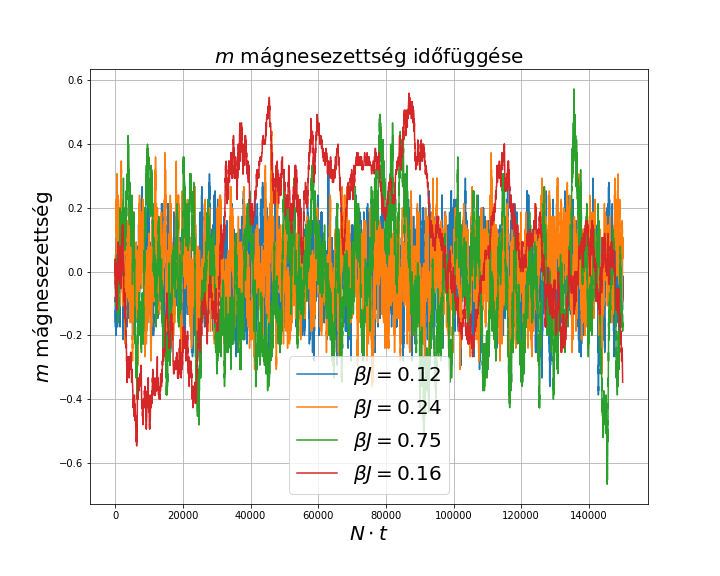
\includegraphics[width=0.6\textwidth]{m.png}
	\end{center}
\caption{Az m mágnesezettség időfüggése a különböző $\beta J$ értékek mellett.}
\label{m}
\end{figure}

\begin{figure}[h!]
	\begin{center}
		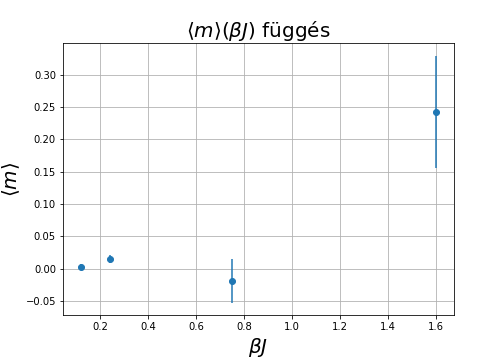
\includegraphics[width=0.6\textwidth]{matlag.png}
	\end{center}
	\caption{Átlagos $\langle m \rangle$ mágnesezettség $\beta J$ függése.}
	\label{matlag}
\end{figure}

\begin{figure}[h!]
	\begin{center}
		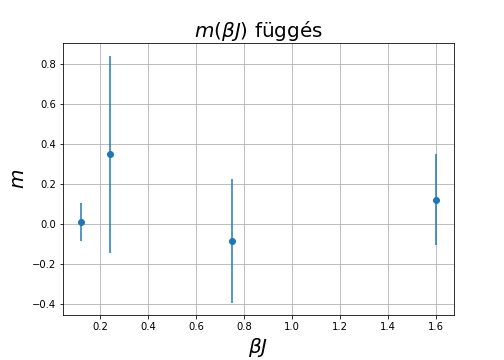
\includegraphics[width=0.6\textwidth]{mm.png}
	\end{center}
	\caption{Végállapoti $m$ mágnesezettség $\beta J$ függése}
	\label{mm}
\end{figure}

\begin{figure}[h!]
	\begin{center}
		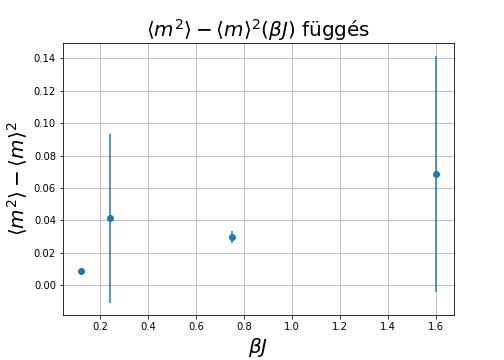
\includegraphics[width=0.6\textwidth]{szorasnegyzet.png}
	\end{center}
	\caption{Átlagos $\langle m^2 \rangle  \langle m\rangle^2 \beta J$ függése.}
	\label{szor}
\end{figure}


\end{document}


